\subsection{Petri Nets}

\subsubsection{Logical And}

\descriptionproblem
Define a Petri Net (P/T net) model for calculating the logical conjunction of two variables, $x$, and $y$, each of which takes the values \emph{true} or \emph{false}, with each variable's value being independent of the other.

\questionproblem
\begin{enumerate}
    \item Draw the diagram describing the aforementioned P/T ned model.

    \item Define a P/T net that computes the negation of $x$, which again takes only the values \emph{true} and \emph{false}.
    
    \item Define a P/T net that computes $!\left(x \land y\right)$ by composing the previous models.
\end{enumerate}

\solution
\textbf{\underline{Solution 1}.} We use a Petri Net (section~\ref{subsubsection: study concurrent use of resources at architectural level (PT Net)} at page~\pageref{subsubsection: study concurrent use of resources at architectural level (PT Net)}) to describe distributed systems. In other words, it is a soft UML graph with an exact mathematical definition of its execution semantics.


The exercise requests that we design a P/T net that describes the logic and operator (conjunction of two variables): $x \land y$. The values of the variables are their domain, \emph{true} and \emph{false}, and then they are boolean values. The values to try depend on the logic table:

\begin{table}[!htp]
    \centering
    \begin{tabular}{@{} c c c @{}}
        \toprule
        $x$ & $y$ & $\land$ \\
        \midrule
        \texttt{True} & \texttt{True} & \texttt{True} \\
        \texttt{True} & \texttt{False} & \texttt{False} \\
        \texttt{False} & \texttt{True} & \texttt{False} \\
        \texttt{False} & \texttt{False} & \texttt{False} \\
        \bottomrule
    \end{tabular}
\end{table}

\noindent
The Petri Net model is exposed in the Figure~\ref{fig: exercises - logical and}.

\begin{figure}[!htp]
    \centering
    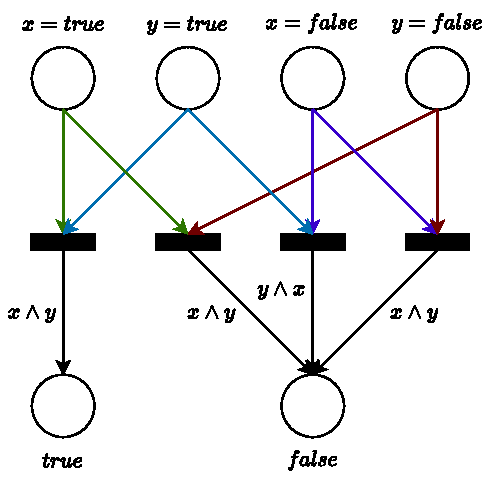
\includegraphics[width=.7\textwidth]{img/logical-and-1.pdf}
    \caption{Petri Net model of logical and.}
    \label{fig: exercises - logical and}
\end{figure}

\highspace
\textbf{\underline{Solution 2}.} The model of the negation $x$ depends on the negation logic table:

\begin{table}[!htp]
    \centering
    \begin{tabular}{@{} c c @{}}
        \toprule
        $x$ & $\lnot x$ \\
        \midrule
        \texttt{True} & \texttt{False} \\
        \texttt{False} & \texttt{True} \\
        \bottomrule
    \end{tabular}
\end{table}

\noindent
The Petri Net model is exposed in the Figure~\ref{fig: exercises - logical not}.

\begin{figure}[!htp]
    \centering
    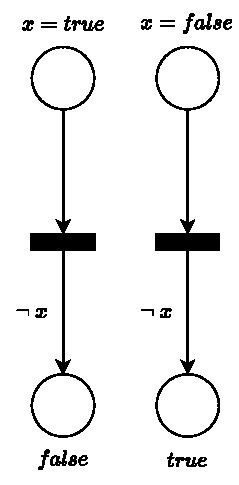
\includegraphics[width=.35\textwidth]{img/logical-and-2.pdf}
    \caption{Petri Net model of logical not.}
    \label{fig: exercises - logical not}
\end{figure}

\highspace
\textbf{\underline{Solution 3}.} To combine the previous two models, we can extend the first model (Figure~\ref{fig: exercises - logical and}) with the second (Figure~\ref{fig: exercises - logical not}) in a very simple way. See the final Petri Net model in the Figure~\ref{fig: exercises - logical and, not}.

\begin{figure}[!htp]
    \centering
    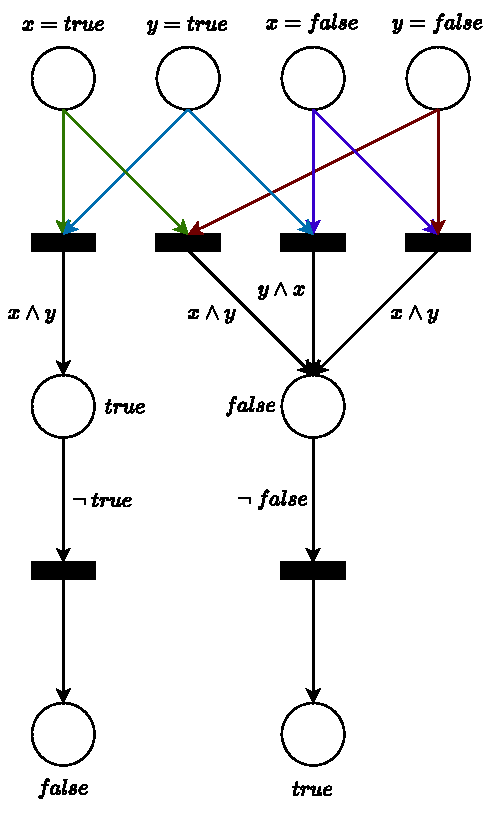
\includegraphics[width=.7\textwidth]{img/logical-and-3.pdf}
    \caption{Petri Net model of logical $\land$ and $\lnot$.}
    \label{fig: exercises - logical and, not}
\end{figure}

\newpage

\subsubsection{Reachability graph}

\descriptionproblem
Consider the P/T Net $\left(N, M0\right)$ presented in Figure~\ref{fig: example of P/T Net model}.

\begin{figure}[!htp]
    \centering
    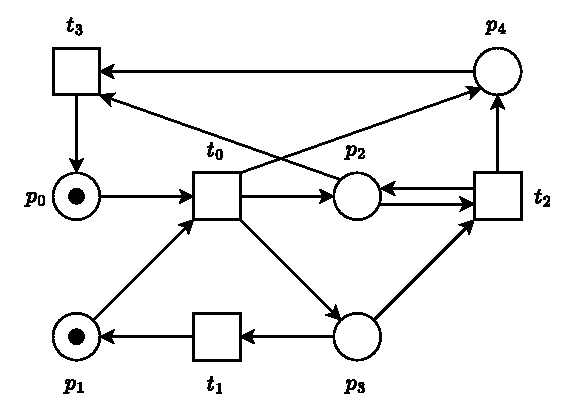
\includegraphics[width=.7\textwidth]{img/reachability-graph-1.pdf}
    \caption{An example of P/T Net model.}
    \label{fig: example of P/T Net model}
\end{figure}

\questionproblem
\begin{enumerate}
    \item Define the reachability graph of $\left(N, M0\right)$.
\end{enumerate}

\solution
\textbf{\underline{Solution 1}.} The reachability graph of the Petri Net:
\begin{enumerate}
    \item The initial state of the model has the state $p_0$ and $p_1$ active. This is the start of the reachability graph: $\left\{p_0, p_1\right\}$.

    \item The arcs leave states $p_0$ and $p_1$ and go to transition 0 ($t_0$). The destinations are $p_2$, $p_3$ and $p_4$. This is the reachability graph:
    \begin{figure}[!htp]
        \centering
        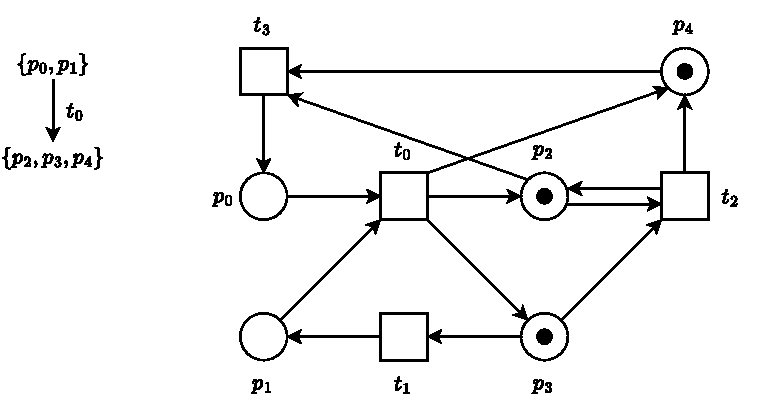
\includegraphics[width=.85\textwidth]{img/reachability-graph-2.pdf}
    \end{figure}

    \newpage

    \item We are evaluating three possible options:
    \begin{itemize}
        \item $t_3$
        \begin{enumerate}
            \item The transition $t_3$ requires the states $p_3$ and $p_4$. The target will be $p_0$:
            \begin{figure}[!htp]
                \centering
                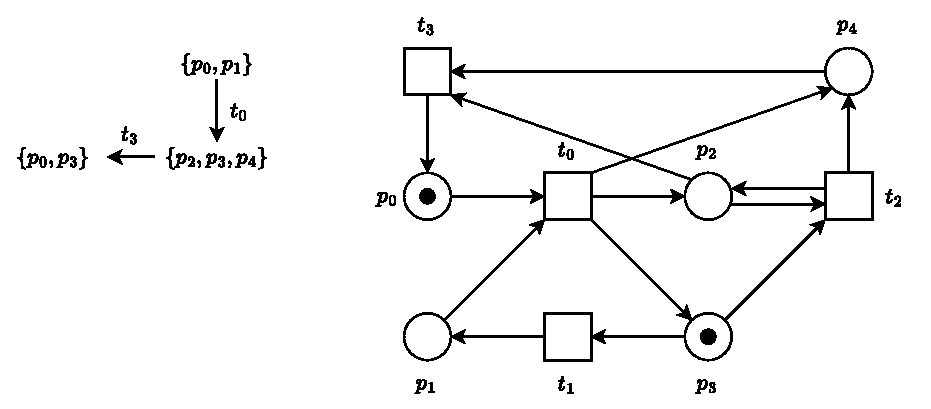
\includegraphics[width=\textwidth]{img/reachability-graph-3.pdf}
            \end{figure}

            \item The transition $t_0$ can't be made by the $p_0$ state because it needs the $p_1$ state. Then the $p_3$ state makes the transition $t_1$ towards the $p_1$ state. At this point we can see that it's the same system as the original one.
            \begin{figure}[!htp]
                \centering
                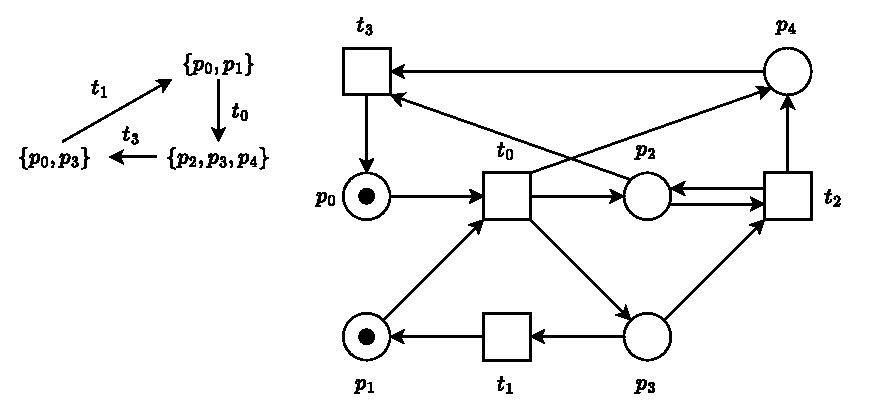
\includegraphics[width=\textwidth]{img/reachability-graph-4.pdf}
            \end{figure}
        \end{enumerate}

        \newpage

        \item $t_1$
        \begin{enumerate}
            \item The transition $t_1$ is made by the state $p_3$. So the destination is $p_1$. 
            \begin{figure}[!htp]
                \centering
                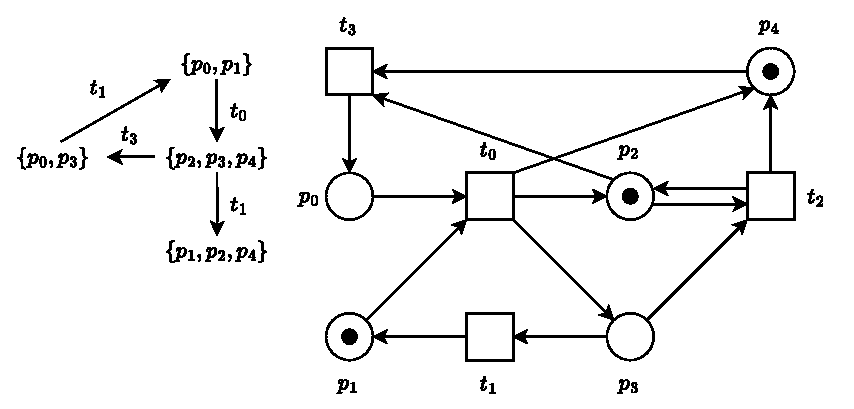
\includegraphics[width=\textwidth]{img/reachability-graph-5.pdf}
            \end{figure}

            \item At this point we can see that the transition $t_0$ cannot be performed by the state $p_1$ because $t_0$ needs the state $p_0$. This state can be performed by the transition $t_3$. Again, this situation brings us back to the initial state.
            \begin{figure}[!htp]
                \centering
                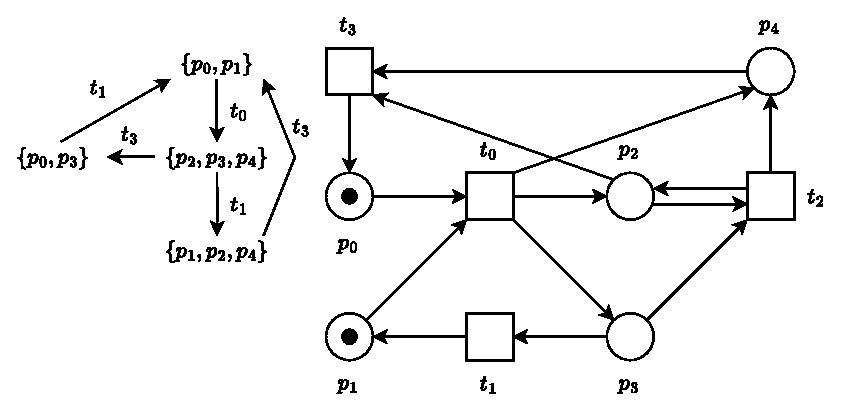
\includegraphics[width=\textwidth]{img/reachability-graph-6.pdf}
            \end{figure}
        \end{enumerate}

        \newpage

        \item $t_2$
        \begin{enumerate}
            \item The transition $t_2$ is made by the state $p_3$ and the state $p_2$. As we can see, the state $p_4$ gets another point and the state $p_2$ doesn't lose its point because it has an internal loop.
            \begin{figure}[!htp]
                \centering
                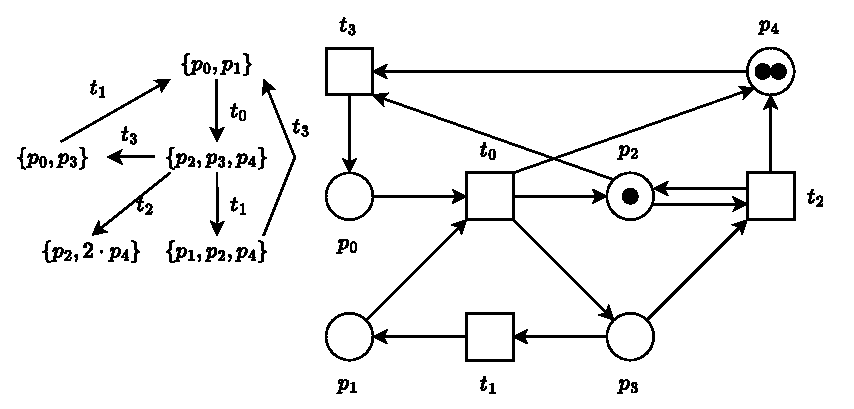
\includegraphics[width=\textwidth]{img/reachability-graph-7.pdf}
            \end{figure}

            \item Finally, we make the transition $t_3$ with $p_2$ and $p_4$.
            \begin{figure}[!htp]
                \centering
                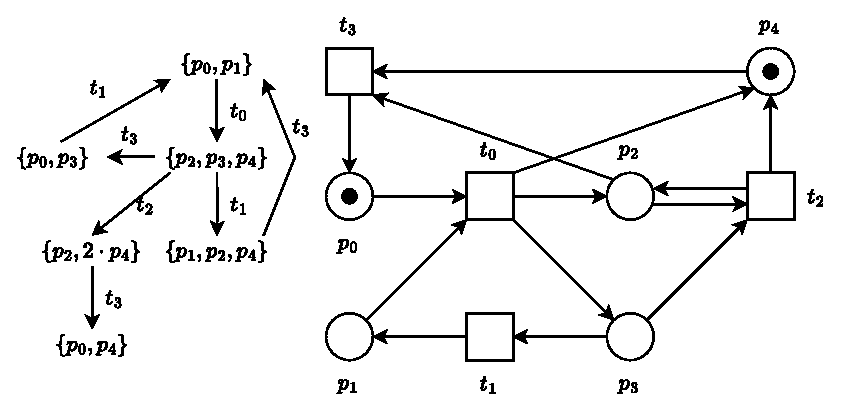
\includegraphics[width=\textwidth]{img/reachability-graph-8.pdf}
            \end{figure}
        \end{enumerate}
    \end{itemize}
\end{enumerate}